\chapter{Системи лінійних рівнянь}


\section{Визначники $n$-го порядку}

Нехай $L$ --- довільний лінійний простір, $e_1, ..., e_n$ --- довільний його базис,
$\dim L = n$. Якщо $x_i \in L$, то $x_i = \sum\limits_{j=1}^n a_{ij} e_j$. Розглянемо
$n$-лінійний кососиметричний нормований функціонал $\varphi(x_1, ..., x_n)$. Тоді $\varphi(e_1, ..., e_n) = 1$.
Узагальнивши співвідношення (2), маємо:

$$\varphi(x_1, ..., x_n) = \sum\limits_{ \begin{pmatrix} 1 & 2 & ... & n \\ i_1 & i_2 & ... & i_n \\ \end{pmatrix} } (-1)^{s(i_1, i_2, ..., i_n)} (a_{1 i_1}, a_{2 i_2}, ..., a_{n i_n}),$$

де $s(i_1, i_2, ..., i_n)$ --- кількість інверсій у $(i_1, ..., i_n)$. 

Нехай $L = \mathbb{R}^n$ і $\{e_1, ..., e_n\}$ --- це канонічний базис. Розглянемо $n$ довільних
векторів з даного простору. Тоді $x_i = \sum\limits_{j=1} a_{ij} e_j$, $i = \overline{1,n}$.
Коефіцієнти розкладу цих векторів утворюють квадратну матрицю порядку $n$: $A = (a_{ij})$, $i,j = \overline{1,n}$.



Озн. Визначником $n$-го порядку називається $n$-лінійний кососиметричний
нормований функціонал, визначений на арифметичному просторі $\mathbb{R}^n$:

$$\det A = \left| \begin{matrix}
	a_{11} & ...    & a_{1n} \\
	\vdots & \ddots & \vdots \\
	a_{n1} & ...    & a_{nn} \\
\end{matrix} \right| = \varphi(x_1, ..., x_n) 
= \sum\limits_{ \begin{pmatrix} 1 & 2 & ... & n \\ i_1 & i_2 & ... & i_n \\ \end{pmatrix} }
	(-1)^{s(i_1, i_2, ..., i_n)} (a_{1 i_1}, a_{2 i_2}, ..., a_{n i_n})$$

де $s(i_1, ..., i_n)$ --- кількість інверсій у перестановці $(i_1, ..., i_n)$. Вказана сума береться
за всіма підстановками $n$-го порядку, тобто $\det A$ є сума добутків $n$ елементів
матриці $A$, які знаходяться в різних рядках та різних стовпчиках, з відповідним
знаком, який визначається кількістю інверсій.

\underline{Властивості визначників $n$-го порядку}

Всі властивості, які було сформульовано для визначників третього порядку,
виконуються і для визначників $n$-го порядку. Це випливає з кососиметричності та
лінійності функціонала $\varphi(x_1, ..., x_n)$.

Нехай $A^T = \{a_{ij}^T\}$ --- це матриця, транспонована до матриці $A$, $a_{ij}^T = a_{ji}$,
$i, j = \overline{1,n}$. Покажемо, що $\det A = \det A^T$.

Оскільки парність підстановок $\begin{pmatrix}
	1 & 2 & ... & n \\
	i_1 & i_2 & ... & i_n \\
\end{pmatrix}$ та $\begin{pmatrix}
	i_1 & i_2 & ... & i_n \\	
	1 & 2 & ... & n \\
\end{pmatrix}$ співпадають, то:

$$\det A^T
= \sum\limits_{ \begin{pmatrix}
				 	1 & 2 & ... & n \\
			 		i_1 & i_2 & ... & i_n \\
				\end{pmatrix} }
	(-1)^{s(i_1, i_2, ..., i_n)} (a_{1 i_1}^T, a_{2 i_2}^T, ..., a_{n i_n}^T)
= \sum\limits_{ \begin{pmatrix}
				 	1 & 2 & ... & n \\
			 		i_1 & i_2 & ... & i_n \\
				\end{pmatrix} }
	(-1)^{s(i_1, i_2, ..., i_n)} (a_{i_1 1}^T, a_{i_2 2}^T, ..., a_{i_n n}^T)
= \det A.$$


\underline{Обчислення визначників $n$-го порядку}

1. Метод пониження порядку грунтується на такому співвідношенні (для фіксованого i ):

$$\det A = \sum\limits_{k=1}^n a_{ik} A_{ik}, (3)$$


де $A_{ik}$ --- це алгебраїчне доповнення елемента $a_{ik}$, яке представляє собою (з точністю
до знаку $(-1)^{i+k}$ визначник $(n-1)$-го порядку, який отримуємо з даного 
визначника викресленням $i$-го рядка та $k$-го стовпчика, на перетині яких
знаходиться елемент $a_{ik}$. Співвідношення (3) називається розкладом визначника
за $i$-им рядком. Аналогічно визначається розклад визначника за певним
стовпчиком. Перед застосуванням методу пониження порядку доцільно,
використовуючи властивості визначника, перетворити в нуль всі, крім одного,
елементи вибраного рядка або стовпчика. Повторивши цю процедуру $(n-2)$ разів,
отримаємо визначник другого порядку, який легко обчислити.

2. Метод зведення до трикутного вигляду полягає в такому перетворенні
визначника, коли всі елементи, розміщені по один бік від головної діагоналі,
дорівнюють нулю. Отриманий трикутний визначник дорівнює добутку елементів
головної діагоналі.


Задача. Обчислити визначник

$$D = \left|\begin{matrix}
	1 & 1 & 1 & 1 \\
	1 & 1 & 2 & 2 \\
	1 & 1 & 1 & 3 \\
	1 & 1 & 1 & 4 \\
\end{matrix} \right|.$$


Розв’язання. Помноживши перший рядок даного визначника на $(-1)$ та
додавши до решти рядків, отримаємо

$$D = \left|\begin{matrix}
	1 & 1  & 1  & 1 \\
	0 & -2 & 1  & 1 \\
	0 & 0  & -2 & 2 \\
	0 & 0  & 0  & 3 \\
\end{matrix} \right| = 1(-2)(-2)3 = 12.$$

\section{Обернена матриця}

Озн. Квадратна матриця $A$ називається невиродженою, якщо $\det A \neq 0$.

Озн. Матрицею, оберненою до $A$ (позн. $A^{-1}$), називається квадратна матриця
$A^{-1}$, для якої виконується рівність $A^{-1} A = A A^{-1} = I$, де $I$ --- це одинична матриця
того ж порядку: $A I = I A = A$.


Лема. Якщо $i \neq j$, то сума добутків елементів $i$-го рядка $\det A$ на алгебраїчне
доповнення $j$-го рядка дорівнює нулю, тобто $a_{j1} A_{j1} + a_{j2} A_{j2} + ... + a_{jn} A_{jn} = 0$.


Доведення. Зауважимо, що алгебраїчне доповнення $A_{ij}$ не залежить ні від
самого елемента $a_{ij}$, ні від інших елементів, що знаходяться в $i$-му рядку та $j$-му
стовпчику визначника. Справді, для побудови $A_{ij}$ потрібно з визначника $n$-го
порядку викреслити саме $i$-й рядок та $j$-й стовпчик. В результаті отримаємо мінор
$M_{ij}$ і за формулою $A_{ij} = (-1)^{i+j}M_{ij}$ знайдемо алгебраїчне доповнення $A_{ij}$.


Розклад визначника за $i$-м рядком має вигляд: $\det A = a_{i1} A_{i1} + a_{i2} A_{i2} + ... + a_{in} A_{in}$.
Розглянемо таку суму $a_{j1} A_{j1} + a_{j2} A_{j2} + ... + a_{jn} A_{jn}$. Цю суму можна
інтерпретувати, як визначник деякої матриці $n$-го порядку $\tilde{A}$, в якій замість $i$-го
рядка стоїть $j$-ий рядок:

$$\tilde{A} = \begin{pmatrix}
	a_{11} & a_{12} & ... & ... & a_{1n} \\
	...    & ...    & ... & ... & ...    \\
	a_{j1} & a_{j2} & ... & ... & a_{jn} \\
	...    & ...    & ... & ... & ...    \\
	a_{j1} & a_{j2} & ... & ... & a_{jn} \\ 
	...    & ...    & ... & ... & ...    \\
\end{pmatrix}$$


Очевидно, що $\det \tilde{A} = 0$. Отже,

$$\sum\limits_{k=1}^n a_{jk} A_{jk} = \left\{ \begin{matrix}
	\det A, & \text{якщо } i = j,    \\
	0       & \text{якщо } i \neq j, \\
\end{matrix} \right\} $$

що і треба було довести.



Теорема. Для того, щоб для матриці $A$ існувала обернена матриця $A^{-1}$,
необхідно і достатньо, щоб матриця $A$ була невиродженою.


Необхідність. Нехай $A^{-1}$ --- це обернена матриця до $A$, тобто $A A^{-1} = I$. Згідно
з властивістю визначника добутку двох матриць маємо
$\det(A A^{-1}) = \det A \det A^{-1} = \det I = 1$. Тому $\det A \neq 0$, тобто матриця A ---
невироджена. 


Достатність. Якщо $\det A \neq 0$, то матрицю $A^{-1}$ можна побудувати за нижче
наведеним алгоритмом.

1. Обчислити $\det A$. Якщо $\det A \neq 0$, то існує $A^{-1}$.

2. Побудувати $A^T$.

3. Замінити кожен елемент транспонованої матриці $A^T$ його алгебраїчним
доповненням та домножити отриману матрицю на $\frac{1}{\det A}$. В результаті отримаємо
матрицю

$$B = \dfrac{1}{\det A} \begin{matrix}
	A_{11}^T & A_{12}^T & ... & A_{1n}^T \\
	...      & ...      & ... & ...      \\
	A_{n1}^T & A_{n2}^T & ... & A_{nn}^T \\
\end{matrix} = \dfrac{1}{\det A} \begin{matrix}
	A_{11} & A_{21} & ... & A_{n1} \\
	...    & ...    & ... & ...    \\
	A_{1n} & A_{2n} & ... & A_{nn} \\
\end{matrix}.$$



Доведемо, що $B = A^{-1}$. Для цього обчислимо добуток $A B$, використавши при
цьому наведену вище лему:

$$AB = \dfrac{1}{\det A} \begin{pmatrix}
	a_{11} & ... & a_{1j} & ... & a_{1n} \\
	...    & ... & ...    & ... & ...    \\
	a_{i1} & ... & a_{ij} & ... & a_{in} \\
	...    & ... & ...    & ... & ...    \\
	a_{n1} & ... & a_{nj} & ... & a_{nn} \\ 
\end{pmatrix}    \begin{pmatrix}
	A_{11} & ... & A_{j1} & ... & A_{n1} \\
	...    & ... & ...    & ... & ...    \\
	A_{1i} & ... & A_{ji} & ... & A_{ni} \\
	...    & ... & ...    & ... & ...    \\
	A_{1n} & ... & A_{jn} & ... & A_{nn} \\ 
\end{pmatrix} = $$

$$= \dfrac{1}{\det A} \begin{pmatrix}
	\det A & ... & 0      & ... & 0      \\
	...    & ... & ...    & ... & ...    \\
	0      & ... & \det A & ... & 0      \\
	...    & ... & ...    & ... & ...    \\
	0      & ... & 0      & ... & \det A \\ 
\end{pmatrix}
= \begin{pmatrix}
	1      & ... & 0      & ... & 0      \\
	...    & ... & ...    & ... & ...    \\
	0      & ... & 1      & ... & 0      \\
	...    & ... & ...    & ... & ...    \\
	0      & ... & 0      & ... & 1      \\ 
\end{pmatrix}
= I.$$


Аналогічно доводиться, що $B A = I$. Отже, $B = A^{-1}$, тобто невиродженість
матриці $A$ гарантує існування оберненої матриці.


\underline{Властивості оберненої матриці}

1. $(\alpha A)^{-1} = \frac{1}{\alpha} a^{-1}$.

2. $(AB)^{-1} = B^{-1} A^{-1}$.

3. $(A^{-1})^T = (A^T)^{-1}$.

\section{Матричний спосіб розв’язування систем лінійних рівнянь}

Розглянемо рівняння $A X = B$, де $A$ --- це квадратна матриця порядку $n$, $B$ ---
це деяка матриця, а $X$ --- це матриця, яку потрібно знайти. Такі рівняння
називаються матричними.

Якщо $\det A \neq 0$, то існує обернена до неї матриця $A^{-1}$. Домножимо обидві
частини даного рівняння зліва на $A^{-1}$:

$$A^{-1} A X = A^{-1} B.$$

Оскільки $A^{-1} A = I$, то отримаємо шукану матрицю:

$$X = A^{-1} B.$$

Зауваження. Якщо задано матричне рівняння $X A = B$, то для знаходження
невідомої матриці X потрібно домножити дане рівняння на $A^{-1}$ справа. Тоді
розв’язок буде мати вигляд: $ X = B A^{-1}$.


Задача. Розв’язати матричним способом систему лінійних рівнянь

$$\left\{ \begin{matrix}
	x + y + z = 2 \\
	2x - y - z = 1 \\
	3x + y - z = -2 \\
\end{matrix} \right..$$

Розв’язання. Використовуючи операцію множення матриць, запишемо дану
систему у матричному вигляді:

$$\begin{pmatrix}
	1 & 1  & 1  \\
	2 & -1 & -1 \\
	3 & 1  & -1 \\
\end{pmatrix} \begin{pmatrix}
	x \\
	y \\
	z \\
\end{pmatrix}
= \begin{pmatrix}
	2 \\
	1 \\
	-2 \\
\end{pmatrix} \text{ або } AX = B.$$

Матриця $A = \begin{pmatrix}
	1 & 1  & 1  \\
	2 & -1 & -1 \\
	3 & 1  & -1 \\
\end{pmatrix} $ називається основною матрицею системи
лінійних рівнянь, $X = \begin{pmatrix}
	x \\
	y \\
	z \\
\end{pmatrix}$ --- це вектор-стовпчик невідомих, а $B = \begin{pmatrix}
	2 \\
	1 \\
	-2 \\
\end{pmatrix}$ --- це
вектор-стовпчик вільних членів. Розв’язок системи знайдемо за формулою
$X = A^{-1} B$. Для цього потрібно обчислити матрицю, обернену до $A$ за наведеним
вище алгоритмом:

$$\det A = \left| \begin{matrix}
	1 & 1  & 1  \\
	2 & -1 & -1 \\
	3 & 1  & -1 \\
\end{matrix} \right|
= \left| \begin{matrix}
	1 & 1  & 1  \\
	3 & 0  & 0  \\
	3 & 1  & -1 \\
\end{matrix} \right|
= 3 \left| \begin{matrix}
	1 &  1 \\
	1 & -1 \\
\end{matrix} \right|
= -3 (-1 -1) = 6 \neq 0.$$

$$A^T = \begin{pmatrix}
	1 & 2  & 3  \\
	1 & -1 & 1  \\
	1 & -1 & -1 \\
\end{pmatrix}, A^{-1} = \dfrac{1}{6} \begin{pmatrix}
	2  & 2  & 0  \\
	-1 & -4 & 3  \\
	5  & 2  & -3 \\
\end{pmatrix}.$$

$$X = \dfrac{1}{6} \begin{pmatrix}
	2  & 2  & 0  \\
	-1 & -4 & 3  \\
	5  & 2  & -3 \\
\end{pmatrix} \begin{pmatrix}
	 2 \\
	 1 \\
	-2 \\
\end{pmatrix} 
= \dfrac{1}{6} \begin{pmatrix}
	 6  \\
	-12 \\
	 18  \\
\end{pmatrix}
= \begin{pmatrix}
	 1  \\
	-2 \\
	 3  \\
\end{pmatrix}.$$

Отже, розв’язок системи рівнянь має вигляд: $x = 1$, $y = -2$, $z = 3$.

\section{Формули Крамера}

Виведемо явні формули для розв’язання системи $n$ рівнянь з $n$ невідомими.

Нехай система лінійних рівнянь записана у матричному вигляді: $A X = B$,
причому матриця $A$ є квадратною і $\Delta = \det A \neq 0$. Тоді єдиним розв’язком цієї
системи у матричному вигляді є $X = A^{-1} B$. Це означає, що

$$\begin{pmatrix}
	x_1 \\
	... \\
	x_i \\
	... \\
	x_n \\
\end{pmatrix}
= \dfrac{1}{\Delta} \begin{pmatrix}
	A_{11} & ... & A_{n1} \\
	...    & ... & ...    \\
	A_{11} & ... & A_{n1} \\
	...    & ... & ...    \\
	A_{11} & ... & A_{n1} \\
\end{pmatrix} \begin{pmatrix}
	b_1    \\
	~      \\
	\vdots \\
	~      \\
	b_n    \\
\end{pmatrix}.$$



Згідно з правилом множення матриць маємо

$$x_i = \dfrac{1}{\Delta}(b_1 A_{1i} + ... + b_n A_{ni}) = \dfrac{\Delta_i}{\Delta}, i = i, ..., n,$$

де

$$\Delta_i = \left| \begin{matrix}
	a_{11} & ... & a_{1, i-1} & b_1    & a_{1,i+1} & ... & a_{1 n} \\
	& & & & & & \\
	\vdots & ... & \vdots     & \vdots & \vdots & ... & \vdots     \\
	& & & & & & \\	
	a_{n1} & ... & a_{n, i-1} & b_n    & a_{n,i+1} & ... & a_{n n} \\
\end{matrix} \right| = b_1 A_{1i} + ... + b_n A_{ni}.$$

Тобто $\Delta_i$ --- це визначник матриці, яка отримана з основної матриці заміною $i$-го
стовпчика $(i = 1, ..., n)$ на стовпчик вільних членів.

Правило Крамера: якщо визначник основної матриці системи лінійних рівнянь
$\Delta = \det A \neq 0$, то система є сумісною і має єдиний розв’язок, який знаходиться за
формулою

$$x_i = \dfrac{\Delta_i}{\Delta}, i = 1, ..., n.$$

\section{Ранг матриці}  % p. 85

Нехай задана прямокутна матриця $A$ розміру $m \times n$:

$$ A = \begin{pmatrix}
	a_{11} & ... & a_{1j} & ... & a_{1n} \\
	a_{21} & ... & a_{2j} & ... & a_{2n} \\
	...    & ... & ...    & ... & ...    \\
	a_{i1} & ... & a_{ij} & ... & a_{in} \\
	...    & ... & ...    & ... & ...    \\
	a_{m1} & ... & a_{mj} & ... & a_{mn} \\
\end{pmatrix} $$


Цю матрицю можна розглядати, як набір рядків $\overleftarrow{a}_i = (a_{i1}, a_{i2}, ..., a_{in})$, $i = 1, ..., m$ і
як набір стовпчиків $\overrightarrow{a}_j = \begin{pmatrix}
	a_{1j} \\
	a_{2j} \\
	\vdots \\
	a_{mj} \\
\end{pmatrix} $, $j = 1, ..., n$, де $\overleftarrow{a}_i \in \mathbb{R}^n$, 
$\overrightarrow{a}_i \in \mathbb{R}^m$. Тоді матриця $A$
може бути подана у вигляді:

$$A = \begin{pmatrix}
	\overleftarrow{a}_1 \\
	\overleftarrow{a}_2 \\
	\vdots \\
	\overleftarrow{a}_m \\
\end{pmatrix}  = (\overleftarrow{a}_1, \overleftarrow{a}_2 ..., \overleftarrow{a}_m).$$


Ранг матриці вводиться по аналогії з поняттям рангу системи векторів.

Озн. Рангом матриці $A$ (позначається $\rang A$) називається ранг системи
векторів, яку утворюють її рядки або стовпчики.

Очевидно, що $\rang A \leqslant \min(m,n)$. Зауважимо, що ранги системи векторів-рядків
та системи векторів-стовпчиків співпадають. Цей факт є наслідком методу
обвідних мінорів, який буде наведено нижче. Знаходити ранг матриці можна двома
способами.

\textit{Метод елементарних перетворень (зведення до трапецоїдного вигляду)}

Метод елементарних перетворень грунтується на наступних твердженнях.


Тв. 1. Ранг матриці не змінюється, якщо поміняти місцями рядки чи
стовпчики.


Тв. 2. Ранг матриці не зміниться, якщо до рядка чи стовпчика додати лінійну
комбінацію інших рядків чи стовпчиків.


Тв. 3. Якщо $\overleftarrow{x}_1 = (a_{11}, a_{12}, ..., a_{1k}, ..., a_{1n})$, 
$\overleftarrow{x}_2 = (0, a_{22}, ..., a_{2k}, ..., a_{2n})$, ..., 
$\overleftarrow{x}_k = (0, 0, ..., a_{kk}, ..., a_{kn})$ і $a_{11} a_{22} ... a_{kk} \neq 0$, то
вектори $\overleftarrow{x}_1, \overleftarrow{x}_2, ..., \overleftarrow{x}_k$ є лінійно
незалежними.


Доведення проведемо від супротивного. Нехай вектори $\overleftarrow{x}_1, \overleftarrow{x}_2, ..., \overleftarrow{x}_k$ є лінійно
залежними. Це означає, що існують числа $\alpha_1, ..., \alpha_k$, $\sum\limits_{i=1}^k |\alpha_i| \neq 0$
такі, що $\alpha_1 \overleftarrow{x}_1 + ... + \alpha_k \overleftarrow{x}_k = \overleftarrow{0}$.
Помноживши вектор $\overleftarrow{x}_i$ на $\alpha_i$ і просумувавши за $i = 1, ..., k$,
маємо

$$(\alpha_1 a_{11}, \alpha_1 a_{12}, ..., \alpha_1 a_{1k}, ..., \alpha_1 a_{1n})
	+ (0, \alpha_2 a_{22}, ..., \alpha_2 a_{2k}, ..., \alpha_2 a_{2n}) + ...$$

$$	+ ...
	+ (0, 0, ..., \alpha_k a_{kk}, ..., \alpha_k a_{kn})
= (\alpha_1 a_{11}, \alpha_1 a_{12} + \alpha_2 a_{22}, ..., $$

$$\alpha_1 a_{1k } + \alpha_2 a_{2k} + ... + \alpha_k a_{kk}, ..., \alpha_1 a_{1n} + \alpha_2 a_{2n} + ... + \alpha_k a_{kn})
= (0, 0, ..., 0, .., 0).$$


Таким чином, маємо:

$\alpha_1 a_{11} = 0, a_{11} \neq 0 \Rightarrow \alpha_1 = 0,$

$\alpha_1 a_{12} + \alpha_2 a_{22} = \alpha_2 a_{22} = 0, a_{22} \neq 0 \Rightarrow \alpha_2 = 0.$

Аналогічно доводимо, що $\alpha_3 = 0, ..., \alpha_k = 0$. Отримане протиріччя і доводить
твердження 3 про лінійну незалежність векторів $\overleftarrow{x}_1, \overleftarrow{x}_2, ..., \overleftarrow{x}_k$.

Таким чином, щоб знайти ранг деякої матриці, потрібно застосувати
елементарні перетворення (див. твердження 1 – 3) та звести її до трапецоїдного
вигляду. При цьому ранг матриці дорівнює кількості ненульових елементів на
похилій бічній стороні трапеції.


Задача. Знайти ранг матриці $A$ методом елементарних перетворень:

$$A = \begin{pmatrix}
	2 & -1 & 3 & -2 & 4 \\
	4 & -2 & 5 &  1 & 7 \\
	2 & -1 & 1 &  8 & 2 \\
\end{pmatrix}.$$


Розв’язання. Помножимо перший рядок даної матриці на (-2) та додамо до
другого рядка, далі домножимо перший рядок матриці на (-1) та додамо до
третього рядка. Переставимо місцями другий та третій стовпчики (знак $\sim$
використовуємо для позначення рівності рангів відповідних матриць):

$$\begin{pmatrix}
	2 & -1 & 3 & -2 & 4 \\
	4 & -2 & 5 &  1 & 7 \\
	2 & -1 & 1 &  8 & 2 \\
\end{pmatrix} \sim \begin{pmatrix}
	2 & -1 &  3 & -2 &  4 \\
	0 &  0 & -1 &  5 & -1 \\
	0 &  0 & -2 & 10 & -2 \\
\end{pmatrix} \sim \begin{pmatrix}
	2 &  3 & -1 & -2 &  4 \\
	0 & -1 &  0 &  5 & -1 \\
	0 & -2 &  0 & 10 & -2 \\
\end{pmatrix}.$$


Домноживши другий рядок отриманої матриці на (-2) та додавши до третього
рядка, отримаємо матрицю у трапецоїдному вигляді, причому на похилій стороні
трапеції стоять ненульові числа --- їх два, тобто $\rang A = 2$:

$$\begin{pmatrix}
	2 &  3 & -1 & -2 &  4 \\
	0 & -1 &  0 &  5 & -1 \\
	0 &  0 &  0 &  0 &  0 \\
\end{pmatrix} \Rightarrow \rang A = 2.$$

\section{Метод обвідних мінорів}

Нехай матриця $A$ --- це прямокутна матриця $m \times n$.

$$A = \begin{pmatrix}
	a_{11} & ...    & a_{1n} \\
	\vdots & \ddots & \vdots \\
	a_{m1} & ...    & a_{mn} \\
\end{pmatrix}.$$


Озн. Мінором $k$-го порядку називається визначник квадратної матриці $k \times k$,
яка утворена перетином $k$ рядків і $k$ стовпчиків матриці $A$.


Озн. Обвідним мінором для мінора $k$-го порядку називається мінор порядку
$(k + 1)$, який містить всі елементи мінора $k$-го порядку.


Наприклад, для матриці з попередньої задачі $a_{11} = 2$ – це мінор першого
порядку. Обвідними для цього мінору є

$$\left| \begin{matrix}
	2 & -1 \\
	4 & -2 \\
\end{matrix} \right|, \left| \begin{matrix}
	2 & 3 \\
	4 & 5 \\
\end{matrix} \right|, \left| \begin{matrix}
	2 & 3 \\
	2 & 1 \\
\end{matrix} \right| \text{ і т.п.}$$


Для мінора $\left| \begin{matrix}
	2 & 3 \\
	4 & 5 \\
\end{matrix} \right|$ обвідними будуть мінори

$$\left| \begin{matrix}
	2 & -1 & 3 \\
	4 & -2 & 5 \\
	2 & -1 & 1 \\
\end{matrix} \right|, \left| \begin{matrix}
	2 & 3 & -2 \\
	4 & 5 & -1 \\
	2 & 1 & -8 \\
\end{matrix} \right|, \left| \begin{matrix}
	2 & 3 & 4 \\
	4 & 5 & 7 \\
	2 & 1 & 2 \\
\end{matrix} \right|.$$


Зауважимо, що існує $C_3^3 C_5^3 = 1 \frac{5!}{3!2!} = 10$ мінорів третього порядку, які
можна побудувати з елементів цієї матриці.


Тв. 1. Якщо вкорочені стовпчики матриці є лінійно незалежними, то і повні
стовпчики також є лінійно незалежними. 


Тв. 2. Якщо повні стовпчики матриці є лінійно залежними, то і вкорочені
стовпчики також є лінійно залежними.


Теорема. Ранг матриці $A$ дорівнює порядку ненульового мінора, всі обвідні
якого є нульовими або їх не можна побудувати.


Доведення. Розташуємо рядки і стовпчики матриці $A$ таким чином, щоб
ненульовий мінор $k$-го порядку був розташований у лівому верхньому куті:

$$A = \begin{pmatrix}
	\mathbf{a_{11}} & ... & \mathbf{a_{1k}} & ...    & a_{1j} & ... & a_{1n} \\
	\vdots          &     & \vdots          & \ddots &        &     & \vdots \\
	\mathbf{a_{k1}} & ... & \mathbf{a_{kk}} & ...    & a_{kj} & ... & a_{kn} \\
	\vdots          &     &                 & \ddots &        &     & \vdots \\
	a_{m1}          & ... & a_{mk}          & ...    & a_{mj} & ... & a_{mn} \\
\end{pmatrix}.$$

Позначимо

$$d = \left| \begin{matrix}
	a_{11} & ...    & a_{1k} \\
	\vdots & \ddots & \vdots \\
	a_{k1} & ...    & a_{kk} \\
\end{matrix} \right| \neq 0.$$


Нехай $\overrightarrow{a}_1, ...,\overrightarrow{a}_k, ..., \overrightarrow{a}_j$ --- це
стовпчики матриці, де $j \in \{k+1, ..., n\}$ ---
фіксований номер стовпчика. Перші $k$ стовпчиків є лінійно незалежними, тому що
вкорочені стовпчики визначника $d$ є лінійно незалежними (див. твердження 1).

Доведемо, що стовпчик $\overrightarrow{a}_j$ можна лінійно виразити через перші $k$ стовпчиків.
Це і буде означати, що $k$ --- це максимальна кількість лінійно незалежних
стовпчиків, тобто $\rang A = k$.


Побудуємо визначник $(k + 1)$ порядку:

$$D = \left| \begin{matrix}
	a_{11} & ... & a_{1k} & a_{1j} \\
	...    & ... & ...    & ...    \\
	a_{k1} & ... & a_{kk} & a_{kj} \\
	a_{i1} & ... & a_{ik} & a_{ij} \\
\end{matrix} \right|, k+1 \leqslant j \leqslant n, 1 \leqslant i \leqslant m.$$


Якщо $i = 1, ..., k$ то $D = 0$ тому, що відовідна матриця має два однакових
рядки. Якщо ж $i > k$, то $D = 0$ тому, що тому, що $D$ --- це обвідний мінор для
вказаного мінора $k$-го порядку.

Розкладемо $D$ за останнім рядком

$$D = a_{i1} A_{k+1, 1} + a_{i2} A_{k+1, 2} + ... + a_{ik} A_{k+1, k} + a_{ij} d = 0.$$

Тоді

$$a_{ij} d = -A_{k+1,1} a_{i1} -A_{k+1,2} a_{i2} -... -A_{k+1,k} a_{ik}$$

або

$$a_{ij} = \alpha_1 a_{i1} + \alpha_2 a_{i2} + ... + \alpha_k a_{ik},$$

де $\alpha_l = -A_{k+1,l}/d$, $l = 1, ..., k$. При цьому враховано,що коефіцієнти $A_{k+1,1}$, $A_{k+1,2}$, ...,
$A_{k+1,k}$, від $i$ не залежать. Останній вираз означає координатний запис
співвідношення:

$$\overrightarrow{a}_{j} = \alpha_1 \overrightarrow{a}_1 + \alpha_2 \overrightarrow{a}_2 + ... + \alpha_k \overrightarrow{a}_k,$$


тобто довільний стовпчик матриці $A$, який стоїть за “межами” квадрата розміру
$k \times k$, можна виразити через перші $k$ стовпчиків. Таким чином, стовпчики $\overrightarrow{a}_1$, ...,
$\overrightarrow{a}_k$, $\overrightarrow{a}_j$ є лінійно залежними, отже $\rang A = k$. Теорему доведено.



Наслідок 1. Ранг системи векторів, яку утворюють рядки матриці, дорівнює
рангу системи векторів, яку утворюють стовпчики матриці.


Дане твердження випливає з того, що обчислення рангу зводиться до
обчислення визначників, які, як відомо, не змінюються при транспонуванні
матриці.


Наслідок 2. Якщо $A$ --- квадратна матриця розміру $k \times k$ і $\det A \neq 0$, то
стовпчики (рядки) є лінійно незалежними.


Задача. Знайти ранг матриці методом обвідних мінорів

$$A = \begin{pmatrix}
	2 & -1 & 3 & -2 & 4 \\
	4 & -2 & 5 &  1 & 7 \\
	2 & -1 & 1 &  8 & 2	\\
\end{pmatrix}.$$

Розв’язання. Оберемо довільний ненульовий мінор першого порядку:
$M_1 = |-1| \neq 0 \Rightarrow \rang A \geqslant 1$. Побудуємо обвідний мінор для $M_1$:

$$M_2 = \left| \begin{matrix}
	-1 & 3 \\
	-2 & 5 \\
\end{matrix} \right| =  1 \neq 0 \Rightarrow \rang A \geqslant 2.$$

Далі будуємо обвідний мінор для M2:

$$M_3^{(1)} = \left| \begin{matrix}
	2 & -1 & 3 \\
	4 & -2 & 5 \\
	2 & -1 & 1 \\
\end{matrix} \right| = 0.$$

Оскільки $M_3^{(1)} = 0$, то будуємо інший обвідний мінор для M2:

$$M_3^{(2)} = \left| \begin{matrix}
	-1 &  3 & -2 \\
	-2 &  5 &  1 \\
	-1 & -1 &  8 \\
\end{matrix} \right| = 0.$$

Будуємо третій і останній з обвідних мінорів:

$$M_3^{(3)} = \left| \begin{matrix}
	-1 &  3 & 4 \\
	-2 &  5 & 7 \\
	-1 & -1 & 2 \\
\end{matrix} \right| = 0.$$

Оскільки не існує ненульових обвідних мінорів третього порядку для $M_2$, то
$\rang A = 2$.

\section{Системи лінійних рівнянь}

Озн. Системою $m$ лінійних рівнянь з $n$ невідомими $x_1$, $x_2$, ..., $x_n$ називається
система, яка має вигляд:

$$\begin{array}{l}
	a_{11} x_1 + a_{12} x_2 + ... + a_{1n} x_n = b_1, \\
	a_{21} x_1 + a_{22} x_2 + ... + a_{2n} x_n = b_2, \\
	\vdots \\
	a_{m1} x_1 + a_{m2} x_2 + ... + a_{mn} x_n = b_m. \\
\end{array}$$

де $A = \begin{pmatrix}
	a_{11} & ...    & a_{1n} \\
	\vdots & \ddots & \vdots \\
	a_{m1} & ...    & a_{mn} \\
\end{pmatrix}$ --- це матриця системи, а $\overline{b} = \begin{pmatrix}
	b_1 \\
	\vdots \\	
	b_m \\
\end{pmatrix}$ --- стовпчик вільних членів.


Якщо $\overline{x} = \begin{pmatrix}
	x_1 \\
	\vdots \\	
	x_n \\
\end{pmatrix}$, то систему можна переписати в матричному вигляді так:

$$ A \overline{x} =  \overline{b}.$$


Озн. Система називається сумісною, якщо вона має розв’язок, в
протилежному випадку --- несумісною. Якщо $\overline{b} = \overline{0}$, то система називається
однорідною, якщо ж $\overline{b} \neq \overline{0}$, то маємо неоднорідну систему рівнянь.

\section{Однорідні системи лінійних рівнянь}

Розглянемо лінійну систему однорідних рівнянь:

$$\begin{matrix}
	a_{11} x_1 + ... + a_{1k} x_k + a_{1,k+1} x_{k+1} + ... + a_{1n} x_n = 0, \\
	\vdots \\
	a_{11} x_1 + ... + a_{1k} x_k + a_{1,k+1} x_{k+1} + ... + a_{1n} x_n = 0, \\
	\vdots \\
	a_{11} x_1 + ... + a_{1k} x_k + a_{1,k+1} x_{k+1} + ... + a_{1n} x_n = 0, \\
\end{matrix} (*)$$

де де $A = \begin{pmatrix}
	a_{11} & ...    & a_{1n} \\
	\vdots & \ddots & \vdots \\
	a_{m1} & ...    & a_{mn} \\
\end{pmatrix}$ --- це матриця системи. Якщо $\rang A = k$, то можна,
переставляючи рівняння і невідомі, вважати, що ненульовий мінор $k$-го порядку,
розташовано у лівому верховному куті матриці $A$, тобто $\left| \begin{matrix}
	a_{11} & ...    & a_{1k} \\
	\vdots & \ddots & \vdots \\
	a_{k1} & ...    & a_{kk} \\
\end{matrix} \right| \neq 0$. Цей
мінор будемо називати базовим. Тоді зрозуміло, що останні $(m - k)$ рівнянь лінійно
залежать від перших $k$ рівнянь, і їх можна не брати до уваги.


Невідомі $x_1$, ..., $x_k$ називаються незалежними (базовими) змінними, а $x_{k+1}$, ..., $x_n$ ---
параметрами. Тоді

$$\begin{matrix}
	a_{11} x_1 + ... + a_{1k} x_k = -a_{1,k+1} x_{k+1} - ... - a_{1n} x_n, \\
	a_{21} x_1 + ... + a_{2k} x_k = -a_{2,k+1} x_{k+1} - ... - a_{2n} x_n, \\
	\vdots \\
	a_{k1} x_1 + ... + a_{kk} x_k = -a_{k,k+1} x_{k+1} - ... - a_{kn} x_n, \\
\end{matrix} (**)$$


Ця система називається системою базисних рівнянь.


Тв. Система лінійних рівнянь (*) еквівалентна системі базисних рівнянь (**).


В системі базисних рівнянь невідомі $x_1$, ..., $x_k$ єдиним чином виражаються
через $(n - k)$ параметрів $x_{k+1}$, ..., $x_n$ (наприклад, можна скористатись формулами
Крамера). Розв’язок системи (**) запишемо у вигляді:

$$\begin{matrix}
	x_1 = c_{11} x_{k+1} + c_{12} x_{k+2} + ... + c_{1,n-k} x_{n}, \\
	x_2 = c_{21} x_{k+1} + c_{22} x_{k+2} + ... + c_{2,n-k} x_{n}, \\
	\vdots \\
	x_k = c_{k1} x_{k+1} + c_{k2} x_{k+2} + ... + c_{k,n-k} x_{n}, \\
	x_{k=1} = x_{k+1}, \\
	\vdots \\
	x_{n} = x_{n}, \\
\end{matrix} $$


Перепишемо цей розв’язок у векторному вигляді:

$$\begin{pmatrix}
	x_1 \\
	x_2 \\
	\vdots \\
	x_k \\
	x_{k+1} \\
	x_{k+2} \\
	\vdots \\
	x_n \\
\end{pmatrix} = x_{k+1} \begin{pmatrix}
	c_{11} \\
	c_{21} \\
	\vdots \\
	c_{k1} \\
	1 \\
	0 \\
	\vdots \\
	0 \\
\end{pmatrix} + x_{k+2} \begin{pmatrix}
	c_{12} \\
	c_{22} \\
	\vdots \\
	c_{k2} \\
	0 \\
	1 \\
	\vdots \\
	0 \\
\end{pmatrix} + ... + x_{n} \begin{pmatrix}
	c_{1,n-k} \\
	c_{2,n-k} \\
	\vdots \\
	c_{k,n-k} \\
	0 \\
	0 \\
	\vdots \\
	1 \\
\end{pmatrix}.$$

Отриманий вираз називається загальним розв’язком однорідної системи
лінійних рівнянь (*). Вектори, які стоять при параметрах $x_{k+1}$, ..., $x_{n}$ у правій
частині останнього виразу, позначимо $f_1$, $f_2$, ..., $f_{n-k}$. Ці вектори називаються
фундаментальною системою розв’язків однорідної системи (*). Часткові 
розв’язки даної системи можна отримати при конкретних значеннях параметрів.
Тому самі вектори $f_1$, $f_2$, ..., $f_{n-k}$ також є частковими розв’язками.
Складемо із стовпчиків $f_1$, $f_2$, ..., $f_{n-k}$ матрицю розміру $n \times (n - k)$:

$$F = \begin{pmatrix}
	c_{11} & c_{12} & ... & c_{1,n-k} \\
	...    & ...    & ... & ...       \\
	c_{k1} & c_{k2} & ... & c_{k,n-k} \\
	1      & 0      & ... & 0         \\
	0      & 1      & ... & 0         \\
	...    & ...    & ... & ...       \\
	0      & 0      & ... & 1         \\
\end{pmatrix}.$$

За методом обвідних мінорів $\rang F = n - k$, оскільки в $F$ входить одинична
матриця порядку $(n - k)$, визначник якої дорівнює одиниці. Це означає, що вектори
$f_1$, $f_2$, ..., $f_{n-k}$ є лінійно незалежними.


Висновок. Із виду загального розв’язку однорідної системи лінійних рівнянь
випливає, що загальний розв’язок є лінійною оболонкою векторів $f_1$, $f_2$, ..., $f_{n-k}$,
тобто множина всіх розв’язків є лінійним підпростором простору $\mathbb{R}^n$, причому
базисом у цьому підпросторі є вектори $f_1$, $f_2$, ..., $f_{n-k}$, а його розмірність дорівнює
$(n - k)$.


\textit{Алгоритм знаходження розв’язків однорідної системи лінійних рівнянь}


Розглянемо однорідну систему з m лінійних рівнянь з n невідомими.

1. Записуємо основну матрицю $A$ системи та знаходимо $\rang A$ методом
обвідних мінорів. Нехай $\rang A = k$.

2. Викреслюємо $(m - k)$ рівнянь, коефіцієнти яких не входять в базовий мінор.

3. До правої частини переносимо $(n - k)$ невідомих, коефіцієнти при яких не
входять в базовий мінор.

4. Знаходимо базові змінні через параметри (для знаходження розв’язку
використовуємо будь-який метод).

5. Записуємо загальний розв’язок. 

6. Виконуємо перевірку: кожний з векторів $f_i$ фундаментальної системи
розв’язків повинен задовольняти всім рівнянням системи (**).


Задача. Знайти ядро лінійного оператора $A: R^3 \rightarrow R^3$, матриця якого в
канонічному базисі має вигляд:

$$A = \begin{pmatrix}
	2 & -3 & 1 \\
	1 &  1 & 1 \\
	3 & -2 & 2 \\
\end{pmatrix}.$$



Розв’язання. За означенням ядра лінійного оператора маємо:

$$\Ker A = \left\{ \overline{x}: \overline{x} = \begin{pmatrix}
	x_1 \\
	x_2 \\
	x_3 \\
\end{pmatrix} \in R^3, A \overline{x} = 0 \right\}.$$

Зі співвідношення $A \overline{x} = 0$ випливає однорідна система лінійних рівнянь:

$\begin{matrix}
	2x_1 - 3x_2 + x_3 = 0, \\
	x_1 + x_2 + x_3 = 0, \\
	x_1 - 2x_2 + 2x_3 = 0. \\
\end{matrix}$

Знаходимо ранг матриці $A$ методом обвідних мінорів:

$$M_1 = |2| \neq 0 \Rightarrow \rang A \geqslant 1,$$

$$M_2 = \left| \begin{matrix}
	2 & -3 \\
	1 &  1 \\
\end{matrix} \right| = 5 \neq 0 \Rightarrow \rang A \geqslant 2,$$

$$M_3 = \left| \begin{matrix}
	2 & -3 & 1 \\
	1 &  1 & 1 \\
	3 & -2 & 2 \\
\end{matrix} \right| = \left| \begin{matrix}
	2 & -5 & -1 \\
	1 &  0 &  0 \\
	3 & -5 & -1 \\
\end{matrix} \right| = 0 \Rightarrow \rang A = 2.$$

Мінор $M_2$ є базовим, тому маємо систему з двох рівнянь:

$\begin{matrix}
	2x_1 - 3x_2 + x_3 = 0, \\
	x_1 + x_2 + x_3 = 0. \\
\end{matrix}$

Згідно з базовим мінором $M_2$ невідомі $x_1$ та $x_2$ є базовими, а $x_3$ є параметром:

$\begin{matrix}
	2x_1 - 3x_2 = -x_3, \\
	x_1 + x_2 = -x_3. \\
\end{matrix}$

Знайдемо розв’язки за формулами Крамера:

$$\Delta = \left|\begin{matrix}
	2 & -3 \\
	1 &  1 \\
\end{matrix}\right| = 5;$$

$$\Delta_1 = \left|\begin{matrix}
	-x_3 & -3 \\
	-x_3 &  1 \\
\end{matrix}\right| = -4x_3, x_1 = \dfrac{\Delta_1}{\Delta} = -\dfrac{4}{5} x_3 ;$$

$$\Delta_2 = \left|\begin{matrix}
	2 & -x_3 \\
	1 & -x_3 \\
\end{matrix}\right| = -x_3, x_2 = \dfrac{\Delta_2}{\Delta} = -\dfrac{1}{5} x_3 ;$$

Запишемо загальний розв’язок системи:

$$\begin{pmatrix}
	x_1 \\
	x_2 \\
	x_3 \\
\end{pmatrix} = \begin{pmatrix}
	- \dfrac{4}{5} x_3 \\
	- \dfrac{1}{5} x_3 \\
	x_3 \\
\end{pmatrix}  = - \dfrac{x_3}{5} \begin{pmatrix}
	4 \\
	1 \\
	-5 \\
\end{pmatrix}.$$

Фундаментальною системою розв’язків є вектор $f = \begin{pmatrix}
	4  \\
	1  \\
	-5 \\
\end{pmatrix}$



Виконаємо перевірку:

$$\begin{matrix}
	2 ~ 4 - 3 ~ 1 - 5 = 0, \\
	4 + 1 - 5 = 0. \\
\end{matrix}$$

Якщо з простору $R^3$ перейти в ізоморфний простір $E^3$, то множині розв’язків
системи можна дати геометричну інтерпретацію:

\parbox{8cm}{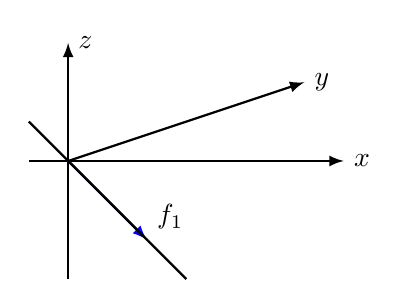
\begin{tikzpicture}[scale=0.5]
	\draw[-latex, thick] (-1,0) -- (7,0)node[right]{$x$};
	\draw[-latex, thick] (0,-3) -- (0,3)node[right]{$z$};
	\draw[-latex, thick] (0,0) -- (6,2)node[right]{$y$};
	\draw[-latex, thick, blue] (0,0) -- (2,-2)node[above right, black]{$f_1$};
	\draw[thick] (-1,1) -- (3,-3);
\end{tikzpicture}}


Отже, розв’язком системи є множина векторів, колінеарних до $f_1$, тобто ядру
лінійного оператора будуть належати вектори простору $E^1$. Базисом ядра є вектор $f_1$.

\section{Неоднорідні системи лінійних рівнянь}

Неоднорідна система з $m$ рівнянь та $n$ невідомими має такий вигляд:

$$\begin{matrix}
	a_{11} x_1 + a_{12} x_2 + ... + a_{1n} x_n = b_1, \\
	a_{21} x_1 + a_{22} x_2 + ... + a_{2n} x_n = b_2, \\
	\vdots \\
	a_{m1} x_1 + a_{m2} x_2 + ... + a_{mn} x_n = b_m, \\
\end{matrix}$$


Матриця $A = \begin{pmatrix}
	a_{11} & ...    & a_{1n} \\
	\vdots & \ddots & \vdots \\
	a_{m1} & ...    & a_{mn} \\
\end{pmatrix} = (\overline{a}_1, \overline{a}_2, ..., \overline{a}_n)$ називається основною
матрицею системи, а матриця $\tilde{A} = \begin{pmatrix}
	a_{11} & ...    & a_{1n} & b_1    \\
	\vdots & \ddots & \vdots & \vdots \\
	a_{m1} & ...    & a_{mn} & b_m    \\
\end{pmatrix} = (\overline{a}_1, \overline{a}_2, ..., \overline{a}_n, \overline{b})$ ---
розширеною матрицею системи. В цих означеннях були використані позначення:

$$\overline{a}_i = \begin{pmatrix}
	a_{1i} \\
	a_{2i} \\
	\vdots \\
	a_{mi} \\
\end{pmatrix}, \overline{b} = \begin{pmatrix}
	b_{1} \\
	b_{2} \\
	\vdots \\
	b_{m} \\
\end{pmatrix} \neq \overline{0}.$$


На відміну від однорідної системи, яка завжди має нульовий розв’язок,
неоднорідна система не завжди є сумісною.


Теорема Кронекера-Капеллі. Неоднорідна система лінійних рівнянь є
сумісною тоді і тільки тоді, коли ранги основної та розширеної матриці
співпадають: $\rang A = \rang \tilde{A}$.

Необхідність. Припустимо, що неоднорідна система лінійних рівнянь є
сумісною. Цю систему можна переписати таким чином: 

$$x_1 \begin{pmatrix}
	a_{11} \\
	a_{21} \\
	\vdots \\
	a_{m1} \\
\end{pmatrix} + x_2 \begin{pmatrix}
	a_{12} \\
	a_{22} \\
	\vdots \\
	a_{m2} \\
\end{pmatrix} + ... + x_n \begin{pmatrix}
	a_{1n} \\
	a_{2n} \\
	\vdots \\
	a_{mn} \\
\end{pmatrix} = \begin{pmatrix}
	b_{1} \\
	b_{2} \\
	\vdots \\
	b_{m} \\
\end{pmatrix}$$

або

$$x_1 \overline{a}_1 + x_2 \overline{a}_2 + ... + x_n \overline{a}_n = \overline{b}.$$

Нехай $\rang A = k$ і саме перші $k$ векторів $\overline{a}_1$, $\overline{a}_2$, ..., $\overline{a}_k$ ---
це максимальна лінійно незалежна підсистема векторів-стовпчиків матриці $A$. Це означає, що
елементи $\overline{a}_{k+1}$, $\overline{a}_{k+2}$, ..., $\overline{a}_{n}$ лінійно виражаються через 
$\overline{a}_1$, $\overline{a}_2$, ..., $\overline{a}_k$. Оскільки
система є сумісною, то вона має розв’язки $\alpha_1$, $\alpha_2$, ..., $\alpha_n$ --- це деякий її розв’язок.
Тоді $\alpha_1 \overline{a}_1 + \alpha_2 \overline{a}_2 + ... + \alpha_n \overline{a}_n = \overline{b}$,
тобто вектор $\overline{b}$ лінійно виражається через $\overline{a}_1$, $\overline{a}_2$, ..., $\overline{a}_k$.
А це і означає, що $\rang A = \rang \tilde{A} = k$.

Достатність. Припустимо, що $\rang A = \rang \tilde{A} = k$. Тобто існують константи
$\beta_1$, $\beta_2$, ..., $\beta_k$ такі, що

$$\overline{b} = \beta_1 \overline{a}_1 + \beta_2 \overline{a}_2 + ... + \beta_k \overline{a}_k
 = \beta_1 \overline{a}_1 + \beta_2 \overline{a}_2 + ... + \beta_k \overline{a}_k + 0 \overline{a}_{k+1} + ... + 0 \overline{a}_{n},$$

тобто $\beta_1$, $\beta_2$, ..., $\beta_k$, 0, ..., 0 є розв’язком неоднорідної системи лінійних рівнянь.
Отже, дана система є сумісною.


\textit{Зв’язок між розв’язками однорідної та неоднорідної систем}


Якщо в неоднорідній системі лінійних рівнянь замінити вільні члени нулями,
то отримаємо однорідну систему, яка називається спряженою системою для
відповідної неоднорідної. Між розв’язками цих систем існує зв’язок, який випливає
із наступного твердження.


Тв. Розв’язком неоднорідної системи є сума загального розв’язку відповідної
однорідної (спряженої) системи та деякого часткового розв’язку неоднорідної
системи. 


Доведення. Нехай $\overline{c} = \begin{pmatrix}
	c_1 \\
	\vdots \\
	c_n \\
\end{pmatrix}$ --- це деякий частковий розв’язок неоднорідної
системи, тобто $A \overline{c} = \overline{b}$, а $\overline{f} = \begin{pmatrix}
	f_1 \\
	\vdots \\
	f_n \\
\end{pmatrix}$ --- це загальний розв’язок відповідної однорідної
системи, тобто $A \overline{f} = \overline{0}$. Тоді $A \overline{c} + A \overline{f} = A(\overline{c} + \overline{f}) = \overline{b}$,
а це і означає, що $\overline{c} + \overline{f}$ є
розв’язком системи $A \overline{x} = \overline{b}$.


Висновок. Загальний розв’язок неоднорідної системи можна отримати, якщо
до будь-якого часткового розв’язку цієї системи додати загальний розв’язок
відповідної однорідної (спряженої) системи.


\textit{Алгоритм знаходження розв’язків неоднорідної системи лінійних рівнянь}


Розглянемо неоднорідну систему з $m$ лінійних рівнянь з $n$ невідомими.

1. Записуємо основну матрицю $A$ системи та розширену матрицю $\tilde{A}$.

2. Знаходимо $\rang A$ та $\rang \tilde{A}$ методом обвідних мінорів.

3. Перевіряємо рівність рангів: $\rang A = \rang \tilde{A}$.

4. Якщо $\rang A < \rang \tilde{A}$, то система є несумісною.

5. Якщо ж $\rang A = \rang \tilde{A} = k$, то викреслюємо $(m - k)$ рівнянь, коефіцієнти яких
не входять в базовий мінор.

6. У праву частину переносимо $(n - k)$ невідомих (параметрів), коефіцієнти при
яких не входять в базовий мінор.

7. Розв’язуємо отриману систему і записуємо загальний розв’язок.

8. Виконуємо подвійну перевірку згідно зі структурою розв’язків неоднорідної
системи.


Задача. Знайти загальний розв’язок системи:

$$\begin{matrix}
	x + 2y + 3z = -4, \\
	2x + 3y + 4z = 1, \\
	3x + 4y + 5z = 6. \\
\end{matrix}$$

Розв’язання. Запишемо основну та розширену матриці:

$$A = \begin{pmatrix}
	1 & 2 & 3 \\
	2 & 3 & 4 \\
	3 & 4 & 5 \\
\end{pmatrix}, \tilde{A} = \begin{pmatrix}
	1 & 2 & 3 & -4 \\
	2 & 3 & 4 & 1 \\
	3 & 4 & 5 & 6 \\
\end{pmatrix}.$$

Знайдемо їх ранги методом обвідних мінорів:

$$M_1 = |1| \neq 0 \Rightarrow \rang A \geqslant 1;$$

$$M_2 = \left| \begin{matrix}
	1 & 2 \\
	2 & 3 \\
\end{matrix} \right| = 3 - 4 = -1 \neq 0 \Rightarrow \rang A \geqslant 2;$$

$$M_3^{(1)} = \left| \begin{matrix}
	1 & 2 & 3 \\
	2 & 3 & 4 \\
	3 & 4 & 5 \\
\end{matrix} \right| = \left| \begin{matrix}
	1 &  0 &  0 \\
	2 & -1 & -2 \\
	3 & -2 & -4 \\
\end{matrix} \right| = 0 \Rightarrow \rang A = 2;$$

$$M_3^{(2)} = \left| \begin{matrix}
	1 & 2 & -4 \\
	2 & 3 & 1 \\
	3 & 4 & 6 \\
\end{matrix} \right| = \left| \begin{matrix}
	1 &  0 &  0 \\
	2 & -1 &  9 \\
	3 & -2 & 18 \\
\end{matrix} \right| = 0 \Rightarrow \rang \tilde{A} = 2;$$


отже $\rang A = \rang \tilde{A} = 2$ і система є сумісною. Виберемо два рівняння, які
відповідають базовому мінору $M_2$, $z$ --- параметр:

$$\begin{matrix}
	x + 2y = -4 -3z, \\
	2x + 3y = 1 -4z. \\
\end{matrix}$$

Позначивши $\Delta = M_2 = -1$ і скориставшись формулами Крамера, маємо

$$\Delta_x = \left| \begin{matrix}
	-4 -3z & 2 \\
	 1 -4z & 3 \\
\end{matrix} \right| = -14 -z, x = \dfrac{\Delta_x}{\Delta} = 14 + z,$$

$$\Delta_y = \left| \begin{matrix}
	1 & -4 -3z \\
	2 &  1 -4z \\
\end{matrix} \right| = 9 + 2z, y = \dfrac{\Delta_y}{\Delta} = -9 -2z.$$

Загальний розв’язок має вигляд:

$$\begin{pmatrix}
	x \\
	y \\
	z \\
\end{pmatrix} = \begin{pmatrix}
	14 + z \\
	-9 - 2z \\
	z \\
\end{pmatrix} = \begin{pmatrix}
	14 \\
	-9 \\
	 0 \\
\end{pmatrix} + z \begin{pmatrix}
	 1 \\
	-2 \\
	 1 \\
\end{pmatrix}.$$

Перевірка полягає в тому, що треба переконатися, що стовпчик $\begin{pmatrix}
	14 \\
	-9 \\
	 0 \\
\end{pmatrix}$ є
частковим розв’язком данної системи, а стовпчик $\begin{pmatrix}
	 1 \\
	-2 \\
	 1 \\
\end{pmatrix}$ --- розв’язком спряженої
системи. 




